% En este capitulo se presentan y analizan los resultados experimentales de la
% solucion para el problema de al exploracion multirobot coordinada que fue
% desarrollada en este proyecto.

% Las pruebas realizadas se separan en tres secciones segun su proposito. La
% primera estudia el impacto de construir el GVD de forma incremental. La
% segunda compara las diversas tecnicas de identificacion de objetivos. Y la
% tercera analiza la influencia de las diversas formas de considerar el espacio
% desconocido. 


% Las pruebas realizadas tienen  propositos,  para estudiar el impacto de
% construir el GVD de forma incremental. Para comparar las diversas tecnicas de
% identificacion de objetivos. Y finalmente para analizar la influencia de las
% diversas formas de considerar el espacio desconocido. 

% , se presentan los resultados obtenidos y analizan
%  los resultados los cuales son analizados.

% Comentar que estos son cosas generales a todas las pruebas, que en cada una de
% las siguientes secciones se cambian paramtros aislados con el proposito de
% comparar su impacto. (ver capaz que crierios se van a comparar en cada una)

% generales de las pruebas realizadas. Estas 

Este capitulo esta dedicado a describir las pruebas realizadas y analizar los
resultados obtenidos. Las pruebas se ejecutaron de forma simuladas y consisten
en resolver una instacia del problema de la exploracion multirobot coordinada.
Los resultados de las pruebas separan en tres secciones segun su proposito. En
la seccion \ref{sec:exp:inc} se estudia el impacto de construir el GVD de forma
incremental. En la seccion \ref{sec:exp:idobj} se compara las diversas tecnicas
de identificacion de objetivos. Y finalmente, en la seccion \ref{sec:exp:desco}
se analiza la influencia de las diversas formas de considerar el espacio
desconocido. 

\section{Especificación de las pruebas}

A lo largo de esta seccion se especifican las pruebas realizadas en este
proyecto.

% * Pruebas realizadas, cosas generales:
%   * simulador
%   * hardware (de mi pc)
%   * Los robots utilizados
%     * sensor 
%     * robot en si
%   * El entorno de pruebas
%   * Criterios utlizados para analizar los resultados: 
%     * Referencias
%     * Explicar cuales son
%   * Cantidad de pruebas, promedio y varianza

% cuyos resultados se
% presentan a lo largo del capitulo.

% En esta seccion se plantean las caracteristicas generales que comparten todas
% las pruebas que se presentan a lo largo del capitulo.

% En lo que resta de esta seccion se especifican las caracteristicas de las
% pruebas llavadas a cabo. 

% A lo largo del capitulo se presentan diversas pruebas que buscan comparar ciertos
% aspectos de la solucion desarrollada en este proyecto. En esta seccion se
% especifican las caracteristicas generales que comparten todas las pruebas
% realizadas.

% En esta sección se establecen als car


% \subsection{Tipos de prueba}
% El proposito de las pruebas presentadas es evaluar el desempeño de diversos aspectos de una
% solucion al problema de la exploción multirobot. 
% Los tipos de prueba quedan definidos 

% Las pruebas tienen como proposito validar las variantes presentadas para la
% solucion de diviersos aspectos de la del problema de exploracion multirobot.
 
% Para lograr esto se definen pruebas consisten en reslover una instancia de
% dicho problema, cambiando la forma de resolver cada aspecto a validar.

% La instancia del problema de exploracion a resolver es el de explorar un
% entorno cerrado con una flota de robots, hasta que no exista espacio sin
% explorar.

% Debido a esto
% las pruebas se dividen en tres secciones, dependiendo del aspecto que se busca comparar.
% Dado esto las pruebas

% En la seccion \ref{sec:exp:inc} se compara la construccion incremental del GVD contra
% la no incremental, en la seccion \ref{sec:exp:idobj} se
% comparan los metodos de identificación de objetivos que se describen en la seccion
% \ref{sec:pc:idobj}, finalmente en la seccion 
%  la seccion \ref{sec:exp:desco} analiza la
% influencia de las diversas formas de considerar el espacio desconocido. 

% de objetivos que
% utiliza directamente las fronteras como objetivos, con las que se basan en
% simplicar dichas fronteras, tanto la simplificacion basada en K-Means, como la
% basada en cubrimiento. 

% Dado que se quiere comparar la utilidad entre las variantes para ciertas partes de
% la solución, se definen tipos de prueba según las variantes utilizadas. 
% En esta sección se describe el tipo de prueba que se denominara como $base$. Este consiste
% en una solucion del problema de exploracion multirobot que 
 % La solución base consiste en resolver la
% asignación de tareas basada en cubrimiento (seccion \ref{subsec:MiSimp}). La as La construccion de GVD
% incremental como es comentada en \ref{sec:MiConstGVD} con

\subsection{Simulador}
Las pruebas fueron simuladas con Gazebo \cite{gazebo}, el cual fue elegido a
partir del analisis comparativo entre varios simuladores candidatos realizado
en la sección \ref{sec:sim}). 

\subsection{Tipos de pruebas}
Las pruebas tienen como proposito validar ciertos aspectos de la
solucion al problema de exploracion multirobot propuesta en este proyecto.
 
Para lograr esto se define caso de prueba que permite evaluar el desempeño de
una solucion que resueve dicho problema. El caso de pruebas definido consiste
en reslover una instancia de dicho problema, especificamente en explorar un
entorno cerrado con una flota de robots, hasta que no exista espacio sin
explorar.

Para poder validar los aspectos, se prueba la solución propuesta cambiando
unicamente el aspecto a validar. Los aspectos a validar son: la construccion
incremental del GVD (sección \ref{sec:MiConstGVD}). La identificación de
objetivos que simplifica las fronteras basandose en el cubrimiento (seccion
\ref{subsec:MiSimp}). Y la consideracion del espacio desconocido al construir
el GVD presentada en la seccion \ref{subsec:espDesc}, donde las celdas
desconocidas no propagan olas y el conjunto $\mli{UF}$ de celdas desconocidas
que son adyacentes a celdas conocidas pertenecen a generadores ($\mli{UF}
\subseteq \mli{CGen}$).

% Para validar la construccion incremental del GVD esta se compara contra la
% construccion no incremental. En el caso de la identificación de objetivos se
% comparan las tres estrategias propuestas en la seccion \ref{sec:pc:idobj}: el
% identificar las fronteras como objetivos, simplicar dichas fronteras a partir
% K-Means, y simplificarlas basandose en el cubrimiento. Por ultimo, la
% consideracion del espacio desconocido en la contruiccion del GVD se valida
% comparandola contra considerar que el espacio desconocido es libre. 
Para validar la construccion incremental del GVD esta se compara contra la
construccion no incremental. En el caso de la identificación de objetivos esta se
comparan contra identificar todas las fronteras como objetivos, y la tecnica
que obtiene los objetivos simplicando dichas fronteras a partir K-Means. Por
ultimo, la consideracion del espacio desconocido en la contruiccion del GVD se
valida comparandola contra considerar que el espacio desconocido es libre. 

Se evaluan entonces cinco soluciones, la que utiliza todos los aspectos a
validar a la vez, y cada una de las que cambian uno de dichos aspectos.

Con el motivo de probar distintas cargas computacionales, cada prueba se repite
cambiando la granularidad de la grilla de ocupacion utlizada para representar
el entorno explorado. La granularidad se indica a traves de las celdas de una
grilla que se corresponden con un metro cuadrado de la realidad. Los valores de
granularidad utilizados para las pruebas son $1,4,9$ y $16$ celdas
por metro cuadrado ($c/m^2$). 

Adicionalente debido a que es posible que ejecuciones de un misma simulacion
lleven a distintos resutlados, con el fin de obtener resultados
estadísticamente significativos cada prueba fue ejecutada 20 veces. Siendo 
$5*4*20=400$ el total de pruebas ejecutadas.
% las tres tecnicas, identfica todas las fornteras como objetivos, 

% Debido a esto
% las pruebas se dividen en tres secciones, dependiendo del aspecto que se busca comparar.
% Dado esto las pruebas

% Para cumplir con la hipotesis (IV) planteada en \ref{sec:hip}
\subsection{Entorno}
Las pruebas se realizan en un entrono cerrado que tiene un area explorable de
aproximadamente $10000m^2$. El entorno esta estructurado en habitaciones,
puertas y corredores de varios tamaños. Los unicos obstaculos presentes en él
son paredes y los mismos robots que pueden obstaculizarse entre
sí. Un mapa de este entrono se muestra en la figura
\ref{fig:willow}.

\begin{figure}[H]
  \center
  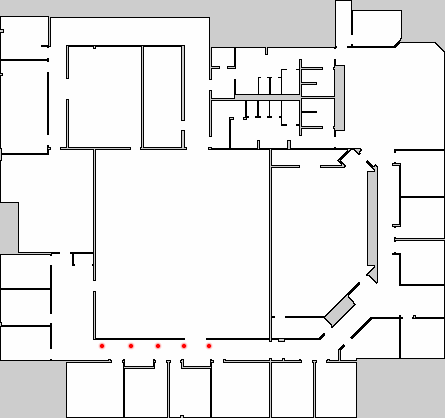
\includegraphics[width=0.5\linewidth]{imagenes/willow/0_250000mRobots2.png}
  \caption[Mapa del entrono utilizado en las pruebas.]{Mapa del entrono utilizado en las pruebas. En negro se indican las paredes, en blanco el espacio libre y en gris el espacio Inaccesible. Las posiciones iniciales de los robots se indican en rojo.}
  \label{fig:willow}
\end{figure} 

El entorno fue construido a partir de un modelo que se encuentra disponible por
defecto en Gazebo, llamado \say{Willow Garage}, el cual se modifico para
reducir el area a exporar y que sea cerrado (sin salidas al exterior).

\subsection{Robots}
Los robots simulados en las pruebas modelan al robot diferencial Pioneer 3-DX
\cite{p3dx} (figura \ref{fig:p3dx}). Cada robot esta equipado con un sensor LiDAR basado en el modelo
URG-04LX-UG01 \cite{hokuyo}, que permite tomar medidas de distancia de hasta
$5.6m$, con una frecuencia de aproximadamente $36hz$. Adicionalente el sensor
fue alterado para tomar medidas en los $360$\textdegree al rededor del robot y
para proporcionar medidas perfectas (sin ruido). %\todo{Justificar? Como?}.

\begin{figure}[H]
  \centerfloat

% , c es adyacente a n3, lo que causa un unico segmento.

  \subfloat[Real.]{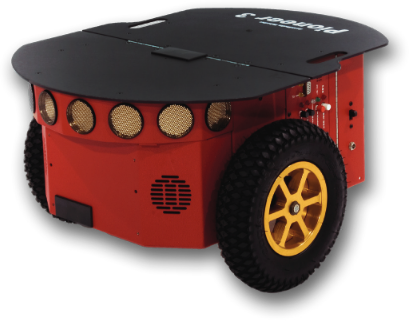
\includegraphics[clip=true, width=0.33\textwidth]{imagenes/pion/real.png}}
  \qquad
  \subfloat[Simulado.]{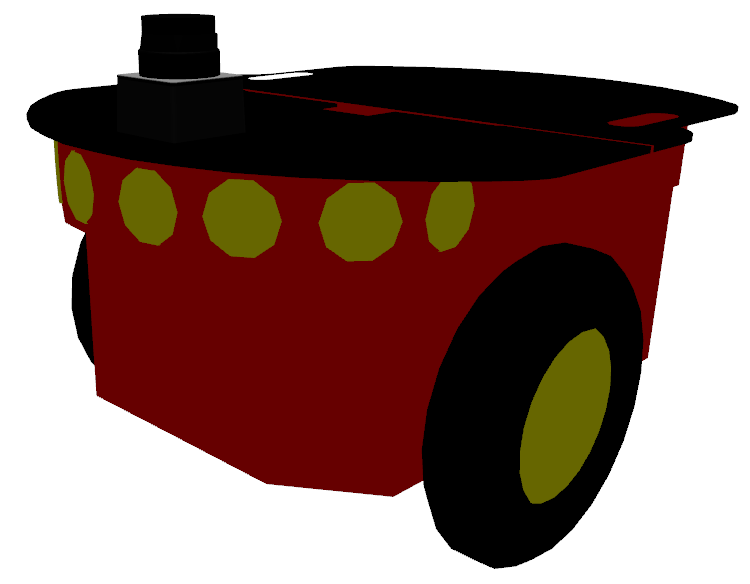
\includegraphics[clip=true, width=0.33\textwidth]{imagenes/pion/sim.png}}

  \caption[Robot diferencial Pioneer 3-DX.]{Robot diferencial Pioneer 3-DX.}\label{fig:p3dx}
   % A la izquierda se muestra el robot real, y a la derecha su version simulada.

\end{figure}

La flota de exploración se compone de cinco robots, ubicados en las posiciones
indicadas en la figura \ref{fig:willow}. Las comunicaciones entre los robots de
la flota son sin perdida y de rango infinito.

\subsection{Hardware}
El simulador junto al resto de procesos necesarios para llevar a cabo una
prueba fueron ejecutados en una computadora personal equipada con un procesador
Intel Core i3-9100F, un procesador gráfico GeForce GTX 660 y 16GB de memoria
RAM.

\section{Metricas}
Las metricas que fueron utilizadas para evaluar y comparar el desempeño de la
exploracion en las pruebas, se basan en las que se proponen en
\cite{yan2015metrics}.



\section{Resultados}
Los resultados explerimentales obtenidos son presentados y analizados en esta
seccion.
\subsection{Incrementalidad}\label{sec:exp:inc}
Los resutlados obtenidos se presentan en la tabla X, y las figuras YZW

\begin{table}[H]
%29/12/2021 18:15:42
\hbadness = 10000
\tolerance=9999
\emergencystretch=10pt
\hyphenpenalty=10000
\exhyphenpenalty=100
\begin{center}

% \begin{adjustbox}{minipage=0.75\paperwidth, center}
\begin{adjustbox}{width=1\textwidth}
\small

\begin{tabularx}{\textwidth}{|X|C{0.80cm}|X|X|X|}

\hline
Construcción del GVD & $\frac{celdas}{m^2}$ & Tiempo de exploración $(s)$ & Distancia total recorrida por la flota $(m)$ & Tiempo promedio en construcción de GVD $(s)$ \\ \hline\hline
\multirow{4}{\linewidth}{\centering Incremental}
& 1 & 463.0±22.6 & 2480.5±109.7 & 0.0442±0.0017\\ \cline{2-5}
& 4 & 496.4±19.0 & 2745.2±107.3 & 0.1762±0.0057\\ \cline{2-5}
& 9 & 549.2±18.4 & 2849.3±95.2 & 0.4204±0.0174\\ \cline{2-5}
& 16 & 678.4±24.8 & 3050.3±105.2 & 0.7641±0.0334\\ \hline\hline
\multirow{4}{\linewidth}{\centering No incremental}
& 1 & 501.9±22.4 & 2653.4±96.5 & 0.7199±0.0122\\ \cline{2-5}
& 4 & 745.7±23.1 & 2851.1±144.0 & 2.8603±0.0484\\ \cline{2-5}
& 9 & 1198.7±35.8 & 3038.1±159.2 & 6.8253±0.1713\\ \cline{2-5}
& 16 & 1856.7±56.2 & 3117.0±170.3 & 12.9256±0.3056\\ \hline
\end{tabularx}
\end{adjustbox}

\caption{Resultados obtenidos en las pruebas realizadas con la construcción incremental y no incremental del GVD.}
\label{tab:inc1}
\end{center}

\end{table}
\todo[inline]{cuadro 4.2: qué tal, Construcción del GVD: incremental vs no incremental}


\begin{table}[H]
%24/12/2021 03:06:44
\hbadness = 10000
\tolerance=9999
\emergencystretch=10pt
\hyphenpenalty=10000
\exhyphenpenalty=100
\begin{center}

% \begin{adjustbox}{minipage=0.75\paperwidth, center}
\begin{adjustbox}{width=1\textwidth}
\small

\begin{tabularx}{\textwidth}{|X|C{0.80cm}|X|X|}

\hline
Construcción del GVD & $\frac{celdas}{m^2}$ & Sumatoria del tiempo en construcción de GVD $(s)$ & Porcentaje del tiempo de obtención de informacion en el que se construye el GVD $(\%)$ \\ \hline\hline
\multirow{4}{\linewidth}{\centering Incremental}
& 1 & 13.48±0.595 & 34.86±1.333\\ \cline{2-4}
& 4 & 45.17±1.489 & 33.80±1.179\\ \cline{2-4}
& 9 & 86.66±2.544 & 34.37±1.124\\ \cline{2-4}
& 16 & 148.25±5.035 & 34.12±1.038\\ \hline\hline
\multirow{4}{\linewidth}{\centering No incremental}
& 1 & 209.31±6.864 & 89.51±0.501\\ \cline{2-4}
& 4 & 477.31±14.931 & 89.33±0.222\\ \cline{2-4}
& 9 & 802.92±29.428 & 89.93±0.203\\ \cline{2-4}
& 16 & 1393.25±45.681 & 89.80±0.309\\ \hline
\end{tabularx}
\end{adjustbox}

\caption{Resultados relacionados a los tiempos de construcción del GVD obtenidos en las pruebas realizadas con la construcción incremental y no incremental del GVD.}
\label{tab:inc2}
\end{center}

\end{table}


\begin{figure}[H]
  \centerfloat

% , c es adyacente a n3, lo que causa un unico segmento.

  \subfloat{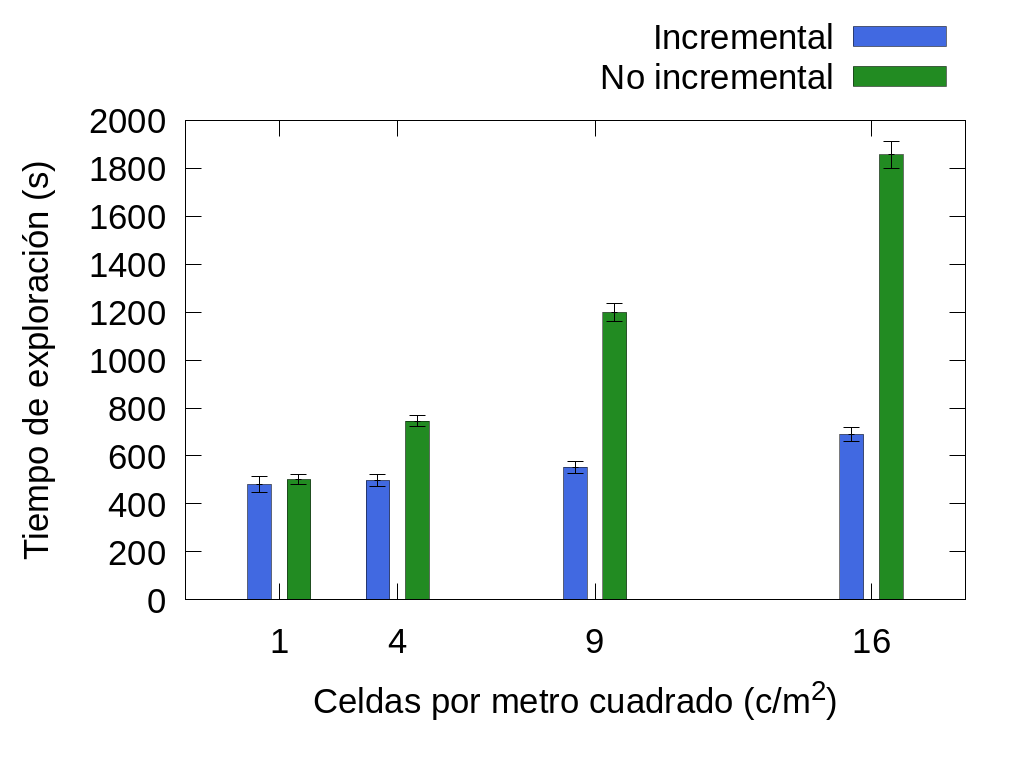
\includegraphics[clip=true, width=0.49\textwidth]{imagenes/graficas_grandes/graficas_histo_num/incrementalidad/exploration_time.png}}
  \qquad
  \subfloat{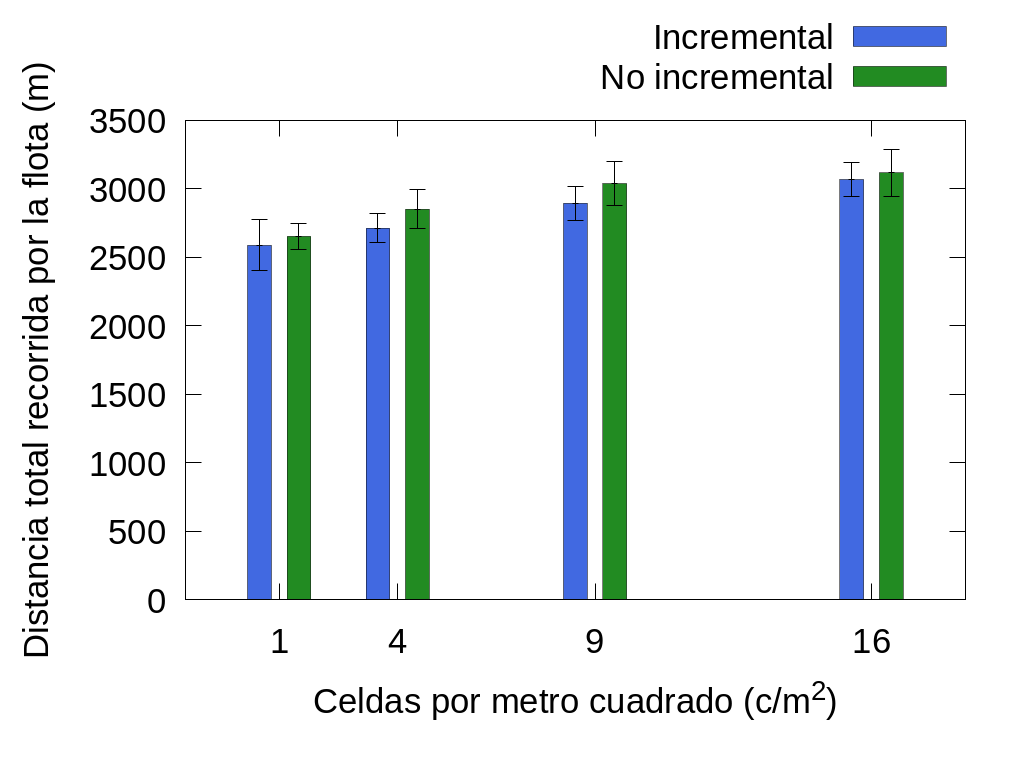
\includegraphics[clip=true, width=0.49\textwidth]{imagenes/graficas_grandes/graficas_histo_num/incrementalidad/exploration_cost.png}}

  \caption[Robot diferencial Pioneer 3-DX.]{Graficas de tiempo de exploración y de distancia total recorrida por la flota, ambas en función de las celdas por metro cuadrado.}\label{fig:gra:inc1}

\end{figure}

\begin{figure}[H]
  \centerfloat

  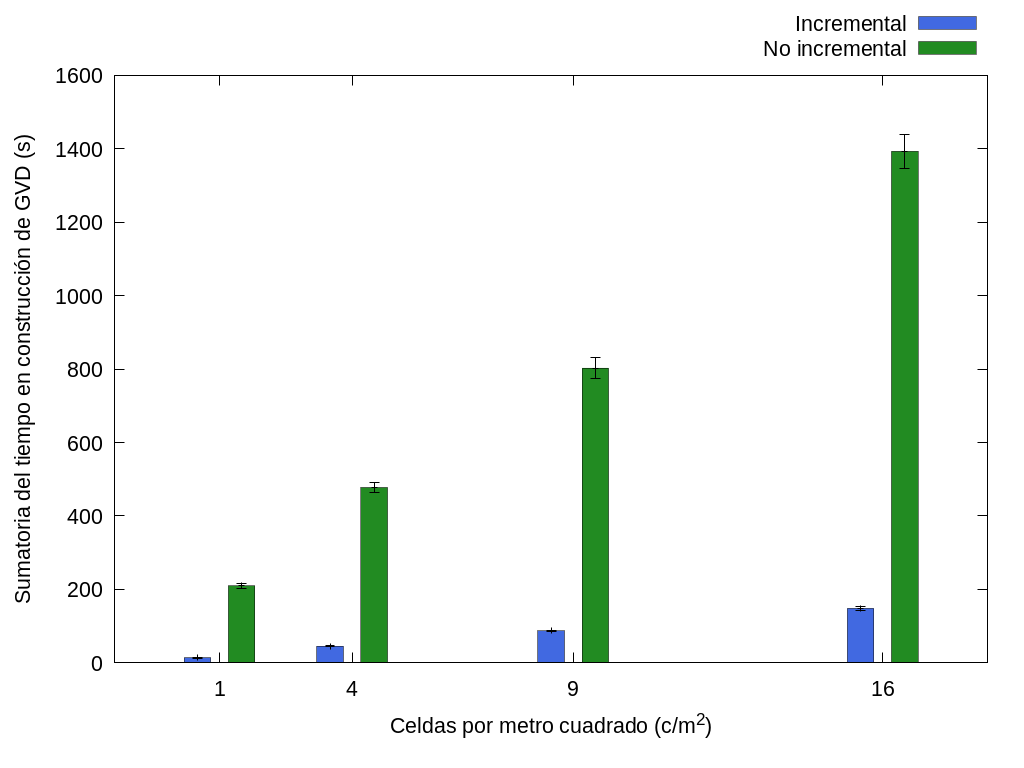
\includegraphics[clip=true, width=0.85\textwidth]{imagenes/graficas_chicas/graficas_histo_num/incrementalidad/gvd_construction_time_sum.png}

  \caption{Grafica de tiempo de exploración en función de las celdas por metro cuadrado.}\label{fig:gra:incs3}

\end{figure}

\begin{figure}[H]
  \centerfloat

  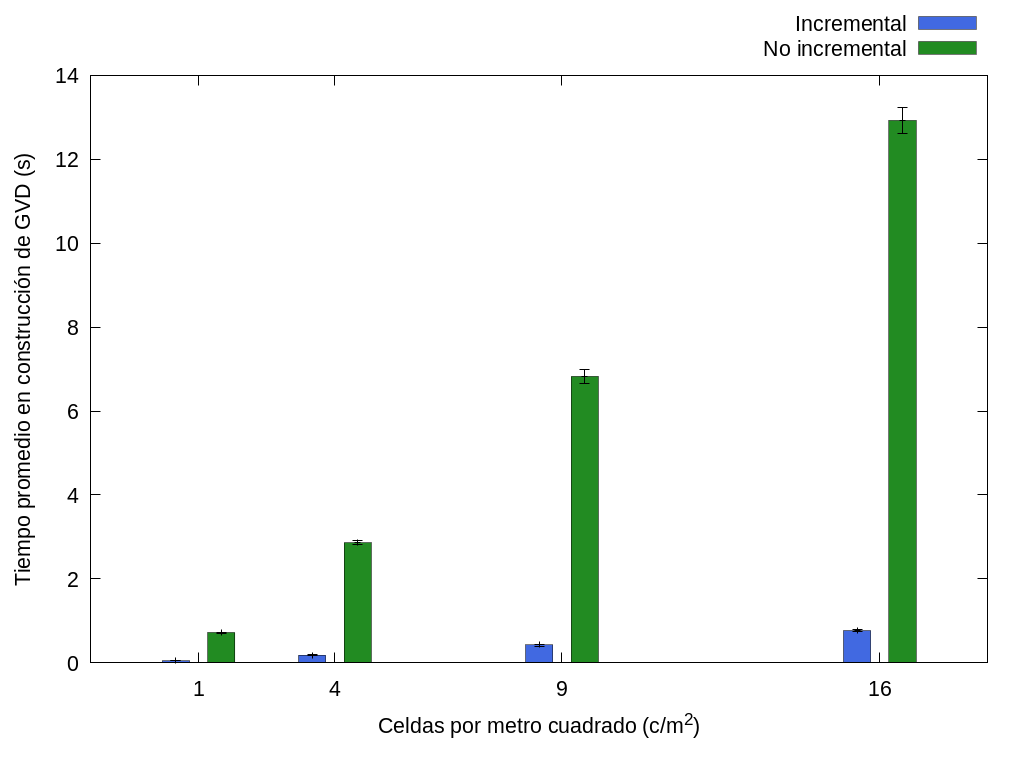
\includegraphics[clip=true, width=0.85\textwidth]{imagenes/graficas_chicas/graficas_histo_num/incrementalidad/gvd_construction_time_mean.png}

  \caption{Grafica de tiempo de exploración en función de las celdas por metro cuadrado.}\label{fig:gra:inc2}

\end{figure}

\subsection{Identificación de objetivos}\label{sec:exp:idobj}

\subsection{Consideracion del espacio desconocido}\label{sec:exp:desco}

